\chapter{Méthode}
Dans cette partie, nous verrons les différentes étapes de BEMD et les améliorations apportées par FABEMD. Ensuite, nous verrons plus en détail l'implémentation que nous avons fait de FABEMD.

\section{Partie théorique}
Pour décomposer une image $I$ en ses différentes fonctions modales intrinsèques, BEMD effectue à chaque la décomposition $i$ d'une image source $S_i$ en son BIMF $F_i$. $S_i$ est l'image résiduelle obtenue telle que $S_i = S_{i-1}-F_{i-1}$ et $S_i = I$.
$F_i$, quant à elle, est obtenue après plusieurs itérations. Les images intermédiaires obtenues à chaque itération $j$ seront désignées par $F_{T_j}$. Les étapes de l'algorithme peuvent ensuite être décrites de la façon suivante :

\begin{algorithmic}
\State $i \gets 1$
\State $S_i \gets I$
\Repeat
	\State $j \gets 1$
	\State $F_{T_j} \gets S_i$
	\Repeat
		\State $P_j \gets maximums(F_{T_j})$
		\State $U_{E_j} \gets interpolation(P_j)$
		\State $Q_j \gets minimums(F_{T_j})$
		\State $L_{E_j} \gets interpolation(Q_j)$
		\State $M_{E_j} = (U_{E_j} + L_{E_j} / 2)$
		\State $F_{T_{j+1}} = F_{T_j} - M_{E_j}$
		\State $D \gets {\sum_{x=1}^{M} \sum_{y=1}^{N} \mid F_{T_{j+1}}(x,y) - F_{T_j}(x,y) \mid^{2} \over \sum_{x=1}^{M}  \sum_{y=1}^{N} \mid F_{T_j}(x,y) \mid^{2}}$
		\State $j \gets j+1$
	\Until{$D < seuil$}
	\State $F_i \gets F_{T_j}$
	\State $i \gets i + 1$
	\State $S_i \gets S_{i-1} - F_{i-1}$
\Until{$nombreExtremums(S_i) < 3$}
\State $R \gets I$
\end{algorithmic}

Comme vu précédemment, FABEMD apporte des améliorations aux étapes de recherches d'extremums et de créations d'enveloppes.
\subsection{Recherche d'extremums locaux}
Pour la recherche d'extremums locaux, FABEMD effectue une recherche de maximum (resp. minimum) pour chaque pixel de l'image. Si la valeur de pixel est strictement supérieure (resp. inférieure) à celle de tous ses voisins, alors le pixel est un maximum local (resp. minimum local). Généralement, le choix d'une fenêtre de recherche de $3x3$ permet d'obtenir les extremums optimaux pour l'image.

\subsection{Création des enveloppes}
Pour la création des enveloppes hautes et basses, FABEMD se base sur les extremums calculés précédemment. Pour chaque point de $P_j$ (resp. $Q_j$), on recherche sa distance à son voisin le plus proche dans $P_j$ (resp. $Q_j$). Ces distances sont stockées dans un tableau d'adjacence de distance des maximums ($d_{adj-max}$) et des minimums ($d_{adj-min}$). Ces distances permettent de déterminer les tailles des fenêtres pour les filtres d'ordre statistique. Il existe ensuite différentes façons de choisir la taille $w_{en-g}$ des fenêtres : celle-ci peuvent être les même pour le filtre de l'enveloppe basse et haute ou non. Cependant les tailles les plus intéressantes sont le minimum des minimums des distances de $d_{adj-max}$ et $d_{adj-min}$ ($d_1$) ou le maximum des maximums des distances de $d_{adj-max}$ et $d_{adj-min}$ ($d_4$).

Ensuite, la valeur de chaque pixel des enveloppe sera la valeur maximale (resp. minimale) dans une fenêtre de taille $w_{en-g}$ autour du pixel. Les enveloppes hautes et basses sont ensuite lissées par un filtre moyenneur de taille $w_{en-g}$.

\section{Implémentation}
Après avoir vu la partie théorique de FABEMD, nous allons voir en détail l'implémentation que nous en avons fait avec la bibliothèque CImg.

\subsection{Analyse UML}
Pour effectuer la décomposition d'une image à l'aide de FABEMD, nous avons créé une classe \texttt{Extrema} pour stocker les extremums de $P_j$ et $Q_j$ ainsi que les distances de $d_{adj-max}$ et $d_{adj-min}$. De plus, une classe \texttt{FABEMD} a été créée pour prendre en charge l'exécution de l'algorithme. L'énumération \texttt{OSFW} a également été créée pour choisir la méthode de choix de taille de filtre. La figure \ref{fig:uml} décrit les interactions entre ces classes.

\begin{figure}[h!]
	\caption{Diagramme UML de l'application}
	\label{fig:uml}
	\centering
	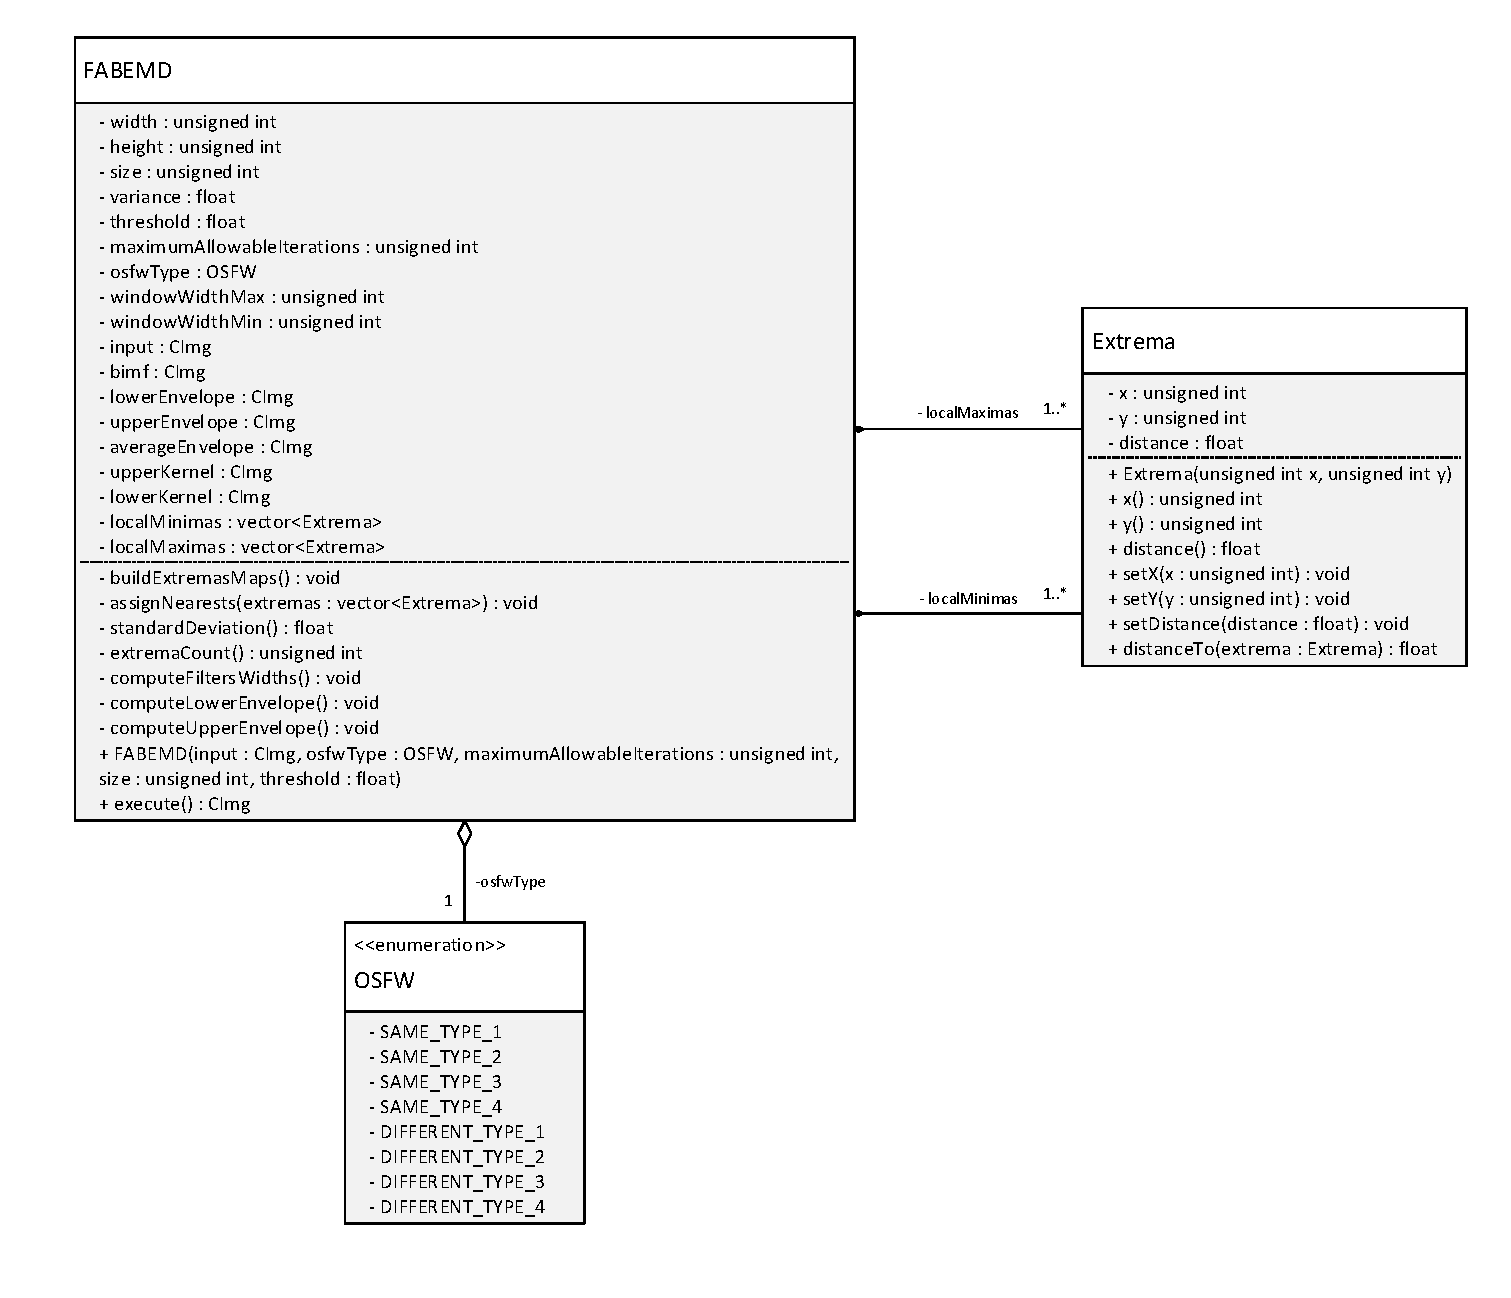
\includegraphics[scale=0.6]{img/uml}
\end{figure}

\subsubsection{Recherche d'extremums}
Pour la recherche d'extremums, la taille de la fenêtre est paramétrable dans le constructeur de \texttt{FABEMD}. Cependant, conserver la taille de 3 est conseillée. La construction s'effectue ensuite dans la méthode \texttt{buildExtremasMaps} et affecte les extremums dans les vecteurs \texttt{localMinimas} et \texttt{localMaximas}.

\subsubsection{Calcul des tailles de filtres}
Une fois les extremums détectés, pour chaque extremum, on recherche la distance à son plus proche voisin avec la méthode \texttt{assignNearests}. L'attribut \texttt{distance} de la classe \texttt{Extrema} stocke cette valeur. Les vecteurs de distance sont ensuite triés selon leur distance et la distance peut être choisie en fonction du \texttt{osfwType} de la classe \texttt{FABEMD} grace à la méthode \texttt{computeFiltersWidths}.

\subsubsection{Calcul des enveloppes}
Une fois les tailles de filtres définies, les enveloppes hautes et basses sont calculés avec la méthode \texttt{computeUpperEnvelope} et \texttt{computeLowerEnvelope}. Pour chaque pixel, on parcourt son voisinage (de taille \texttt{windowWidthMax} (resp. \texttt{windowWidthMin}) et recherche la valeur la plus élevée (resp. la plus faible) qui lui est ensuite affectée. L'enveloppe ainsi créée est convoluée avec le noyau moyenneur \texttt{upperKernel} (resp. \texttt{lowerKernel}) pour effectuer le lissage.

\subsubsection{Stockage des résultats}
Les résultats de l'algorithme (BIMF et résidu) ainsi que l'image originale sont retournés par l'algorithme. L'image originale est contenue à l'indice $z=0$ et est suivie des différents BIMF et enfin du résidu. L'application principale permet de visualiser ces différents résultats en utilisant la molette de la souris sur l'affichage.
